\chapter{The CPSA Search Algorithm}
\label{ch:algorithm}

The result of running the \texttt{cpsa4shape} tool is a file that
contains only ``shapes'', which include all essential structures
possible in executions of the protocol under the conditions input to
the analysis.  Although this output contains the most important
elements of the results of an analysis, it can be useful to an analyst
to examine the full result.

Consider analyzing a protocol that has a secrecy property you wish to
guarantee.  After modeling the protocol, you model a set of conditions
under which you expect the secrecy property to hold, but you include a
listener that would invalidate it.  See Section~\ref{sec:blanchet} for
an instance of the use of this technique.

Suppose the analysis confirms the secrecy property.  This would mean
that there are no shapes at all, because any shape would represent a
possible way in which the conditions were present but the secret is
revealed.  If you look only at the shapes file, you will see nothing
other than the fact that no shapes are present.  The full analysis,
however, can be used to understand the space of attacks that were
explored, which gives a much clearer sense of \emph{why} the analysis
resulted in no shapes.

It is a complicated and somewhat unnatural process modeling a protocol
and setting up the conditions for an analysis.  Human error is
possible, and when a human error occurs, it is difficult for the
analyst---most likely, the human that made the error in the first
place---to distinguish a human error from a correct analysis result.

By examining the full analysis carefully, the analyst may discover
errors of two types: segments of the analysis that seem inconsistent
with the intended scenario, or the \emph{lack} of analysis that the
user expected to be present.  The first circumstance indicates an
analysis that was \emph{under-constrained}, while the latter indicates
one that was \emph{over-constrained}.  In order to detect errors of
the second type, however, the analyst needs to understand the search
algorithm.

Another reason to understand the search algorithm is when the user has
obtained an analysis that describes a genuine attack against a
protocol.  By stepping through the path in the analysis that led to
the shape in question, a user may gain an understanding of what
features of the protocol allowed this attack to take place. This often
leads to insights about how to repair the protocol and eliminate the
attack.

\section{Solving tests}
\label{sec:tests}

\index{skeleton!realized} A \emph{realized} skeleton is one in which
every reception is explainable given the assumed restrictions on the
attacker.  The attacker is capable of producing every basic value
(that is, every possible value of the basic sorts
$\scap{data},\scap{text},\scap{name},\scap{akey},\scap{skey},$ and
$\scap{rndx}$), except for those specifically withheld from the
adversary.  The values withheld are the ones for which there is one of
the following declarations present: \texttt{uniq-orig},
\texttt{uniq-gen}, \texttt{non-orig}, or \texttt{pen-non-orig} (see
Section~\ref{sec:secrecy_assumptions} for detail).

In addition, the attacker observes all of the transmissions made in a
skeleton.  The attacker is also capable of manipulating messages in
certain specific ways -- these are the derivations present in
Table~\ref{tab:basic_algebra_signature}.

When a reception message can be constructed by the attacker from the
basic values accessible to the attacker and the transmissions that
occur prior to that reception, we say it is \emph{realized}, meaning
that this reception can be explained.

When a skeleton to be analyzed contains at least one unrealized node,
one of these nodes is selected as the ``test node'', and the
subsequent skeletons are determined based on four distinct strategies
for resolving (or at least making progress at resolving) the problem
at the test node.  The strategies focus on a \emph{critical term}, a
sub-value of the reception value that is a specific problem for
derivability.  The critical term may be a freshly generated value,
which was generated by a regular participant but is subsequently found
in a different message context than any in which it is known to have
been transmitted.  It may also be an encrypted (or digitally signed)
unit, which must be generated on some regular strand unless the
generating key is compromised.  This inference builds in the
assumption that cryptographic operators have an authentication value,
as a symmetric encryption may be an authenticated encryption.  {\cpsa}
always interprets an encryption operator as guaranteeing authenticity,
unless the key is compromised.

Only certain kinds of sub-values may be of interest as critical terms,
specifically, those which are \emph{carried} \index{carried subterm}.
The notion of a carried sub-term can be defined recursively: a term
carries itself, a pair carries either of its components, and an
encryption carries its plaintext.

The four strategies are:

\begin{itemize}

\index{augmentation!regular}\index{regular augmentation}
\item A \emph{regular augmentation}, which assumes the presence of an
  additional transmission carrying the critical term, in an entirely
  new strand,

\index{displacement}
\item A \emph{displacement}, which assumes the presence of an
  additional transmission carrying the critical term, but in an
  already existing strand,

\index{contraction}
\item A \emph{contraction}, which assumes that the critical issue
  can be resolved with some more refined version of the current
  transmissions that carry the critical value, and

\index{listener augmentation} \index{augmentation!listener}
\item A \emph{listener augmentation}, which assumes that some key
  not known to be derivable is in fact derivable.

\end{itemize}

When examining a skeleton and one of its children in full {\cpsa}
analysis it is often simple to determine which sort of strategy was
used.  If a child has one more strand than its parent then it was
produced by either augmentation (if the extra strand is a role
instance) or listener augmentation (if the extra strand is a
listener).  If a child has the same number of strands but additional
nodes, it is the result of a displacement.  When a child has the same
number of nodes and strands, it may be the result of a displacement or
a contraction, but either way the only thing that has changed is a
map of terms.

\section{Flawed Kerberos, revisited}
\label{sec:kerberos2}
In Section~\ref{sec:kerberos}, we worked through an example -- a
flawed version of the Kerberos protocol.  The first attempt at
modeling the protocol was flawed in a way that would prevent the tool
from discovering the attack against the protocol.

\index{Kerberos protocol}
\index{examples!Kerberos}
See Figure~\ref{fig:kerb-flawed defprotocol} for the flawed model of
the protocol.  Recall that the initiator is $a$, the server is $s$,
and the responder is $b$.  See Figure~\ref{fig:kerb-flawed2
  defprotocol} for the corrected model; the difference is that in the
corrected version, the initiator uses a variable of sort $\scap{mesg}$
to represent the ticket the initiator receives, since the initiator is not
able to check the internal format of the ticket.

\subsection{The operation field}
\label{sec:operation}
\index{operation field} Examining the full {\cpsa} analysis is
essential to detecting the mistake.  Each skeleton has an
\texttt{operation} field describing how it was derived from its
parent, with one exception: when the input skeleton does not meet all
the requirements for a skeleton, the first child will be the minimal
skeleton incorporating the input.

In \texttt{kerb.xhtml}, tree 0 is the flawed model.  Item 0 is the input
point of view and Item 1 is the completion of that input into a
skeleton; notice that the skeleton below Item 1 has no S-expression of
the form \texttt{(operation ...)} in it.

\ttindex{added strand} Item 2 is a child of Item 1 that adds a key
server instance.  This was a regular augmentation, because a new
protocol role instance was added.  The operation field will include
\texttt{added-strand} whenever the skeleton was produced by regular
augmentation.  The full operation field in Item 2 is:

\begin{center}
\verb|(operation encryption-test (added-strand keyserv 2)|\\
\verb|        (enc k n (ltk a s)) (0 1))|
\end{center}

The first argument to the operation field is the general type of
operation performed.  Typically this will be one of the following
three possibilities:

\begin{itemize}
\item \texttt{encryption-test} indicates that the critical term at the
  test node was an encryption.
\item \texttt{nonce-test} indicates that the critical term at the test
  node was an atom, not an encryption.
\item \texttt{channel-test} indicates that the critical term at the test
  node was an authenticated channel message.
\item \texttt{generalization} indicates that the skeleton was realized
  and the tool is trying to make it more general without making it
  unrealized.
\end{itemize}

The second argument describes the operation; here, the operation is
\texttt{added-strand} (regular augmentation), where the new instance
is an instance of \texttt{keyserv} and is of length 2.  The third
argument is the criticial term; here it was \texttt{(enc k n (ltk a s))},
the portion of the server's message intended for the initiator.  The
last argument is a node, normally the test node, so in this case, the
\texttt{(0 1)} refers to strand 0, node 1 -- the second node of the
initiator strand in Item 1.

Returning to our example, Item 2's critical term is the encryption
$\enc{k,n}{SK(a,s)}$.  The regular augmentation creates a new
transmission of that encryption in some carried form; in this case, it
is a transmission by the key server.  Note that the key server
instance in Item 2 agrees with the initiator on $a$ but not on $b$.

See Figure~\ref{fig:kerb-skel3} for Item 3 in the analysis.  It is
this step at which the analyst should notice there was a mistake of
some sort.  If the analyst is trying to understand why it should be
impossible for the secret $m$ to leak, thus far the reasoning is that
if the initiator proceeds to its third event, there is a key server
that agreed with the initiator on $a, s$, and $n$.  But since the
second initiator node is red, this indicates there is still something
unexplained in the execution.

\begin{figure}
\begin{center}
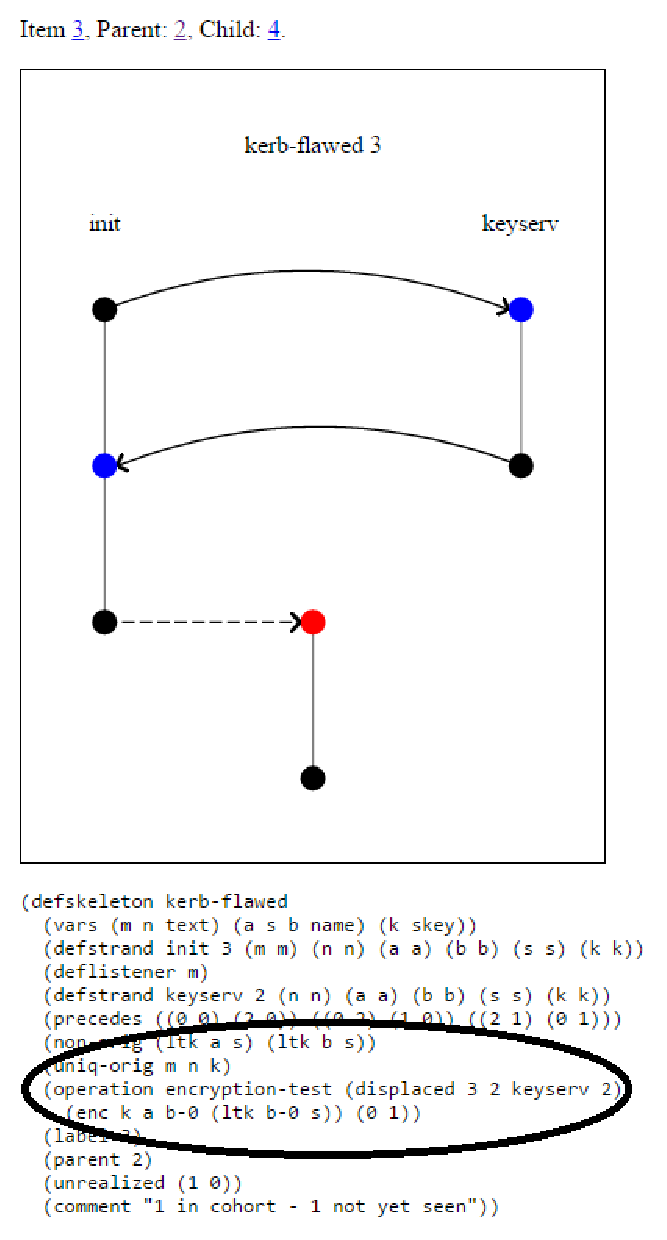
\includegraphics[scale=0.8]{kerb_skel3_operation_circled}
\end{center}
\caption{Flawed Kerberos key moment in analysis}
\label{fig:kerb-skel3}
\end{figure}

The operation field of Item 3 is telling:

\begin{center}
\verb|(operation encryption-test (displaced 3 2 keyserv 2)|\\
\verb|        (enc k a b-0 (ltk b-0 s)) (0 1))|
\end{center}

The critical term here is the encryption $\enc{k,a,b0}{K(b0,s)}$.
Thus, the ticket portion of the initiator's reception is driving this
step in the analysis.\footnote{Note that the specific encryption
  $\enc{k,a,b0}{K(b0,s)}$ is not actually present in Item 2 or in Item
  3, it is a side effect of the internal way {\cpsa} represents
  variables and determines how to display them.  Still, only the
  ticket portion of the node \texttt{(0 1)} is of this kind of format,
  so the conclusion in the text is correct.}  After the displacement
(which, you may notice, adds no new nodes), the key server agrees with
the initiator on $b$.

In other words, the tool reasons first that the presence of the
``authenticator'' portion of the reception guarantees there is a key
server instance that believes it is responding to a request initiated
by $a$, but may or may not believe the request initiated by $a$ was
for communicating with $b$.  The ticket portion makes the guarantee,
but that's strange because the ticket is for $b$ and not $a$ to
examine.  To believe this reasoning implies that the initiator really
is checking the format of the ticket, which the analyst should realize
is not the way the protocol is intended to work.

If you next examine the properly modeled protocol, you will find that
Items 5, 6, and 7 follow a very similar path.  Item 6 makes Item 5 into
a skeleton, while Item 7 adds a key server instance in which the key
server agrees with the initiator on $a$ but not on $b$.  But Item 7 is
a realized skeleton, while Item 2 is not realized.

%%% Local Variables:
%%% mode: latex
%%% TeX-master: "cpsa4manual"
%%% End:
